%%%%%%%%%%%%%%%%%%%% author.tex %%%%%%%%%%%%%%%%%%%%%%%%%%%%%%%%%%%
%
% sample root file for your "contribution" to a contributed volume
%
% Use this file as a template for your own input.
%
%%%%%%%%%%%%%%%% Springer %%%%%%%%%%%%%%%%%%%%%%%%%%%%%%%%%%


% RECOMMENDED %%%%%%%%%%%%%%%%%%%%%%%%%%%%%%%%%%%%%%%%%%%%%%%%%%%
\documentclass[graybox]{svmult}

% choose options for [] as required from the list
% in the Reference Guide

\usepackage{type1cm}        % activate if the above 3 fonts are
                            % not available on your system
%
\usepackage{makeidx}         % allows index generation
\usepackage{graphicx}        % standard LaTeX graphics tool
                             % when including figure files
\usepackage{multicol}        % used for the two-column index
\usepackage[bottom]{footmisc}% places footnotes at page bottom


\usepackage{newtxtext}       % 
\usepackage{newtxmath}       % selects Times Roman as basic font

% see the list of further useful packages
% in the Reference Guide

\makeindex             % used for the subject index
                       % please use the style svind.ist with
                       % your makeindex program

%%%%%%%%%%%%%%%%%%%%%%%%%%%%%%%%%%%%%%%%%%%%%%%%%%%%%%%%%%%%%%%%%%%%%%%%%%%%%%%%%%%%%%%%%

\begin{document}

\title*{Finding the centre: compositional asymmetry in high-throughput sequencing datasets}
% Use \titlerunning{Short Title} for an abbreviated version of
% your contribution title if the original one is too long
\author{Jia R. Wu, Jean M. Macklaim, Briana L. Genge and Gregory B. Gloor}
% Use \authorrunning{Short Title} for an abbreviated version of
% your contribution title if the original one is too long
\institute{Jia R. Wu \at Department of Computer Science, U. Waterloo, Waterloo, Canada, \email{jr2wu@uwaterloo.ca}
\and Jean M. Macklaim \at Department of Biochemistry, London, Ontario, Canada, \email{jean.macklaim@gmail.com}
\and Briana L. Genge \at Department of Biochemistry, London, Ontario, Canada, \email{bgenge3@gmail.com}
\and Gregory B. Gloor,  \at Department of Biochemistry, London, Ontario, Canada, \email{ggloor@uwo.ca}
}
%
% Use the package "url.sty" to avoid
% problems with special characters
% used in your e-mail or web address
%
\maketitle

\abstract*{High throughput sequencing datases comprise millions of reads of genomic data and can be modelled as count compositions. These data are used for transcription profiles, microbial diversity, or relative cellular abundance in culture. The data are sparse, and high dimensional. Moreover, they are often unbalanced: i.e, there is often systematic variation between groups due to presence or absence of features, and this variation is important to the biological interpretation of the data. The imbalance causes samples in the comparison groups to exhibit varying centres contributing to false positive and false negative identifications. Here we extend the centred log-ratio transformation method used for the comparison of univariate differential relative abundance between two groups in a Bayesian compositional context. We demonstrate the pathology in  modelled and real unbalanced experimental designs to show how this causes both false negative and false positive inference. We examined four approaches to identify  denominator features, and tested them with different proportions of modelled asymmetry; two were relatively robust. We recommend the `LVHA' transformation for asymmetric transcriptome datasets, and the `IQLR' method for all other datasets when using the \texttt{ALDEx2} tool available on Bioconductor.}

\abstract{High throughput sequencing datases comprise millions of reads of genomic data and can be modelled as count compositions. These data are used for transcription profiles, microbial diversity, or relative cellular abundance in culture. The data are sparse, and high dimensional. Moreover, they are often unbalanced: i.e, there is often systematic variation between groups due to presence or absence of features, and this variation is important to the biological interpretation of the data. The imbalance causes samples in the comparison groups to exhibit varying centres contributing to false positive and false negative identifications. Here we extend the centred log-ratio transformation method used for the comparison of univariate differential relative abundance between two groups in a Bayesian compositional context. We demonstrate the pathology in  modelled and real unbalanced experimental designs to show how this causes both false negative and false positive inference. We examined four approaches to identify  denominator features, and tested them with different proportions of modelled asymmetry; two were relatively robust. We recommend the `LVHA' transformation for asymmetric transcriptome datasets, and the `IQLR' method for all other datasets when using the \texttt{ALDEx2} tool available on Bioconductor.}

\section{Background}
\label{sec:1}
High throughput sequencing (HTS) technology is used to generate information regarding the relative abundance of features.  In these designs, DNA or RNA is isolated, a library is made from a  sample of the nucleic acid, and a random sample of the library is sequenced on an instrument. The output is a set of short sequence tags, called reads, which are mapped to reference sequences for annotation of each feature that generates a table of read counts per feature for every sample. Traditionally, samples comprise a set of features whose identity depends on the experimental design. For example, features are genes in the case of RNA-sequencing or  metagenomic sequencing, or are operational taxonomic units (OTUs) when the objective is identifying microbial diversity. 
 
The instruments used for HTS have an upper limit on the total number of reads delivered; for example the same library sequenced on an Illumina MiSeq or an Illumina NextSeq will deliver approximately 20 million or 400 million reads. HTS instruments thus deliver a fixed-sum random sample of the sequences that are in the library, which itself is a random sample of what was in the environment \cite{Quinn206425,gloorFrontiers:2017}. It should be obvious that the total number of reads delivered, bears no relationship to the total number of input molecules that was sampled from the environment, and that the only information contained in such data are relative data.

Data from HTS instruments are usually analyzed by count-based methods. For example, the most commonly used tools, edgeR and DESeq2, estimate parameters using  negative binomial models of the data \cite{Robinson:2010,Love:2014aa}. The variance in HTS data is usually larger than the mean (overdispersed), and negative binomial and similar models are generally adequate when the underlying assumptions are approximated \cite{Gierlinski:2015aa}. An important nuance is that  count-based methods must 'correct for library size', that is, adjust the count values in each sample so that all samples have approximately the same total count after normalization. The widely-used scaling normalization correction methods assume that a per-sample midpoint value exists such that the normalization can impute, or at least approximate, the number of each feature in the underlying environment \cite{Robinson:2010a,Dillies:2013}. This per-sample scaling factor is used to scale the count values up or down prior to analysis. Note that scaling-normalization methods do not change the relationships between the features as they are simple linear transformations of all features in a sample \cite{Quinn206425}.

However, many HTS datasets do not provide sensible answers with these statistical models. For example, in meta-transcriptomic datasets the actual and relative abundance of both  organisms and of the genes expressed by the organisms may change independently. The assumption that the majority of features are invariant is broken if there is any sort of systematic variation between groups. When comparing microbial diversity between sampling sites or conditions, organisms present in one sub-site or condition may be absent from another \cite{Macklaim:2015aa,Hummelen:2010,Gajer:2012}. In the case of multi-organism RNA-seq (meta-transcriptomics), organisms resident in one condition may have a different expression profile and abundance than those resident in a second condition \cite{macklaim:2013}. In the case of a single-organism RNA-seq, samples from one condition may express more genes than samples from another condition \cite{Lang:2015aa,Peng:2014aa,Zhao:2013aa,Gierlinski:2015aa}. These differences are represented by either zeroes or low count features that occur systematically in only one group. Such asymmetric datasets are thus some of the most difficult experiments to analyze \cite{macklaim:2013,fernandes:2013} since the datasets do not fit multiple assumptions of existing tools. We have shown previously that existing count-based tools fail to give sensible answers in meta-transcriptome and other datasets that exhibit asymmetry  \cite{fernandes:2013, fernandes:2014,gloorAJS:2016}. 

\subsection*{A ratio based approach to analyzing HTS:}
\label{subsec:1:1}
Another approach to analyze data is to acknowledge the compositional nature of the data, and to examine only relative changes. In this case, we cannot know if the absolute abundances are changing, only if the relationships between features do so. The \texttt{ALDEx2} tool in Bioconductor incorporates this concept by modelling the data as a multivariate probability distribution and by examining the result using the principles of compositional data analysis \cite{Aitchison:1986,fernandes:2013}. Conceptually, the approach is similar to sequencing many different technical replicates of each of the underlying biological replicates, treating the resulting data as ratios of the features and reporting the mean value of the technical replicates. This approach has been found to be a generally useful tool that works for meta-transcriptomic datasets \cite{macklaim:2013} and translates to many different experimental designs \cite{fernandes:2014, mcmurrough:2014,gloorFrontiers:2017,Macklaim:2018aa,Almeida:2019aa}. 

The basis for the approach used by \texttt{ALDEx2} to find univariate differences between groups is the centred log-ratio (CLR) transformation proposed by Aitchison \cite{Aitchison:1986} and defined in equation \ref{eq:CLR} below.  For a given sample, the CLR transformed value of each feature is the logarithm of the ratio between the count of the feature and the geometric mean of the count of all features. Thus, both the feature count and the geometric mean of  all feature counts in the sample affect the value returned after CLR transformation. When comparing features between samples, any systematic change  of either the numerator or the denominator will result in features being apparently different. Given this information, inferences about the relative abundance of the numerator requires some assumptions about the denominator and in the ideal case the denominator should be comparable across all samples. 

We can formally define the problem as follows. We start with compositional vectors $\textbf{x}_i$ and $\textbf{x}_j$ that define the count of samples $i$ and $j$, and our goal is to identify which individual features are distinct in $i$ and $j$. We define $G(\textbf{x}_i)$ as the geometric mean of $\textbf{x}_i$. Then compositional asymmetry is defined as  $G(\textbf{x}_i) \ne G(\textbf{y}_i)$, where the inequality is caused by a systematic and asymmetric difference. 

We note that the constant-denominator assumption is  similar to relative quantitative PCR (qPCR) \cite{Thellin:1999aa,Vandesompele:2002aa}, a method in common use in molecular biology that is often used as the gold-standard to validate HTS results. In this type of qPCR the amount of the unknown feature is determined relative to a standard feature of (presumed) invariant abundance. Within an experiment, the actual amount of the standard does not need to be known, it is sufficient for it to be constant across samples. It is well known that the relative abundance measure will change when a different standard is used as the denominator, leading to the use of multiple (presumed invariant) standards in some cases. Thus, one shortfall of any ratio-based approach, is to determine the appropriate feature(s) to place in the denominator. 

\subsection*{Choosing the denominator:}
\label{subsec1:2}

The basic principle of compositional data analysis as developed by Aitchison is to convert the data into log-ratios between the features for each sample \cite{Aitchison:1986}. Formally, Aitchison defined a composition as a vector \textit{\textbf{x}}  of positive values \textit{x\textsubscript{1}}\ldots\textit{x\textsubscript{D}} whose features  sum to an arbitrary constrained constant $\alpha$. Absolute values of features in a composition are uninformative, and so the only information available in compositional data are the relative magnitudes, or the ratios between the pairs of components. This is the case in HTS since the count observed for a feature contains no information regarding the absolute number of molecules in either the sequencing library or the environment, although the magnitude of the count contains information on the precision of the estimate \cite{gloorAJS:2016,fernandes:2013}.

Data collected from high throughput sequencing are count compositions \cite{fernandes:2014,gloorAJS:2016}. Since all read count totals from a machine are arbitrary we should treat the data as an equivalence class  where the composition contained in vector \textit{\bf{x}} can be scaled into an identical composition \textit{\textbf{y}} by multiplication of a constant $\alpha$ \cite{barcelo:2001}. Thus, in the ideal case, we can discuss any composition as being a probability vector scaled by $\alpha$ without loss of precision \cite{fernandes:2013}. Note that this is similar to the count normalization methods discussed above, but rather than normalizing to a count, we are determining a probability. 

We start with two groups $X$ and $Y$ that are matrices containing samples represented by the vectors $\textbf{x}_1 \dots \textbf{x}_n$ and $\textbf{y}_1 \dots \textbf{y}_m$ with each sample containing the same number of features numbered $1 \dots D$. Our goal is to determine which, if any of the features are reliably different between the groups. 

One way of satisfying the need to examine the ratios between features  in each sample vector is to use the centred-log-ratio (CLR) transformation proposed by Aitchison, defined as: 

\begin{equation}
\textbf{x}_{clr} = log  \Big( \frac{x_{i}}{G(\textbf{x})}   \Big); i=1\dots D
\label{eq:CLR}
\end{equation}

where $G(\textbf{x}) =$ the geometric mean of the D features of  an arbitrary sample in $X$, and similar for samples in $Y$. When interpreting CLR-transformed values, care must be taken  to ensure that the analyst understands that any changes observed are always relative to the denominator of the CLR in each sample. 

%\text{where}~
%	\textbf{x}_{clr} &= \text{A composition transformed by CLR} \\
%	x_i &= \text{A feature of the non-transformed composition (\textbf{x})} \\
%	D &= \text{The number of features of \textbf{x}} \\ 
%	}

The CLR, and any other ratio-based method has the advantage of being sub compositionally dominant for distances, and is, at least in theory, scale-invariant because if the parts of \textit{\textbf{x}} are counts with $\alpha=$\textit{N} reads, then: 

\begin{equation}
	\textbf{x}_{clr}= log\Big( \frac{\alpha x_i}{G(\alpha \textbf{x})}   \Big) =  log\Big( \frac{x_i}{G(\textbf{x})}  \Big).
\label{eq:equip}
\end{equation}

The  important caveat that limits this ideal situation when dealing with high throughput sequencing data is that the total read count, $\alpha$, for each sample should be similar. While the CLR is essentially normalizing for read depth, it does not account for  the uncertainty of measurement at the margins \cite{gloorAJS:2016,fernandes:2013}.
The CLR is the default denominator used by \texttt{ALDEx2}. In practical terms \texttt{ALDEx2} handles the problem of varying read depth by constructing a posterior probability distribution of the original count matrix \cite{fernandes:2013}.  In this approach features in low-count samples have broader probability distributions than features in high-count samples. Thus, the precision of the estimates vary when samples have different read depths.

Aitchison \cite{Aitchison:1986} also defined the ALR, the additive log-ratio as: 

\begin{equation}
\textbf{x}_{alr} = log  \Big( \frac{x_{i}}{x_D}   \Big) ; i=1\dots D-1
\label{eq:ALR}
\end{equation}

where, following from above, $\textit{\textbf{x}}_{alr}$ is the composition of an arbitrary sample from $X$ transformed by ALR. When using the ALR  the denominator is the $D^{th}$ feature of \textit{\textbf{x}}, which by convention in a molecular analysis, such as qPCR, would be a feature assumed to be constant. 

The ALR and CLR can be viewed as the two limits of a continuum of incomplete knowledge about an internal standard by which relative abundance should be judged in order to properly identify differentially abundant features. The ALR uses one presumed constant feature as the denominator; while the CLR  presumes that the majority of features are not changed, leading to the use of the geometric mean of all features as the denominator. Clearly, neither of these are expected to be satisfactory in every case. We can however, choose to use combinations of other features as the basis for comparison.

\subsection*{HTS data are sparse.}
\label{subsec:1.2}
It is common for HTS data to be sparse, that is, for a given sample to contain features with counts of 0. One limitation of the log-ratio approach is that ratios have no meaning if the denominator contains a 0 value. The sparsity of a sample is affected by the total number of reads obtained for each sample, and by the number of features that the total reads are apportioned between. Each sample in a transcriptome contains between thousands and tens of thousands of features each of which may have a potential dynamic range of over 4 orders of magnitude. In many cases a transcriptome dataset will be composed of several groups, where the expression of a feature (gene) is so low that it is below the detection limit in one group, and very high in another group. The expression of genes in biological systems is linked, and some genes control the expression of other genes, either by increasing or decreasing their relative abundance. Furthermore, the cell has a built-in control system whereby gene expression itself appears to be a composition, that is, the expression levels of all genes in a cell in a given environment are constrained by an absolute upper bound  \cite{Scott:2010}. In eukaryotic cells, the upper bound can be changed with surprisingly small genetic changes \cite{Loven:2012aa}, and changes in the upper bound is a known confounder of transcriptome experiments. In the case of a meta-transcriptome a population of cells  does not necessarily exhibit total gene expression with an upper bound, since the cells themselves can change in both absolute and relative abundance in a mixture. 

The assumption being made when using the CLR transformation to identify features that differ between groups is that most features are either invariant or, at worst, vary at random when comparing the two groups. However, marked asymmetry can break this assumption, and this is the problem being addressed by identifying and using alternate denominators.

\subsection*{Alternative denominators}
\label{subsec:1.3}

The starting point for calculating an alternative denominator is a  CLR transformed  count table using Equation \ref{eq:CLR} sample-wise with a uniform prior of 0.5. The CLR transformed group matrices will be represented by $\mathcal{X,Y}$; i.e., $\mathcal{X} = CLR(X)$ and so on for $\mathcal{Y}$. 

The \textit{IQLR} (interquartile log-ratio) transformation uses as the denominator features with conserved `midpoint' variance across groups. Here, the calculated variance corresponds to the diagonal of the covariance matrix of each  group, and the diagonal is a vector of length $D$. For convenience, $var(\mathcal{X})$ corresponds to the diagonal of  $cov(\mathcal{X})$ and similarly $var(\mathcal{Y)}$ is the diagonal of  $cov(\mathcal{Y})$.   The indices of the  features within the interquartile range, $IQR$, of $var(\mathcal{X})$  and $var(\mathcal{Y})$ are chosen and stored in $\textbf{x}_{idx-IQR}$ and  in $\textbf{y}_{idx-IQR}$. Finally, the geometric mean of the intersect of those indices identify the values in the denominator when calculating the \textit{IQLR}. Thus, for a sample $\textbf{x}$ contained in  $X$, the log ratio values are calculated by using the features in $\textbf{x}$ that correspond to the indices as in equation \ref{eq:iqlr}:

\begin{equation}
\textbf{x}_{ IQLR }= log  \Big( \frac{\textbf{x}_i}{G(\textbf{x}[\textbf{x}_{idx-IQR} \cap \textbf{y}_{idx-IQR}] )}  \Big ) ;i=1 \dots D
\label{eq:iqlr}
\end{equation}

and similarly for samples in $Y$. 

The \textit{LVHA} (low variance high abundance log-ratio) transformation uses as the denominator the intersect of those features that have low variance and high relative abundance in each group. These are chosen as the features that exhibit variance below the first quartile and relative abundance above the third quartile on a per-group basis. Thus, in $\mathcal{X}$, low variance features are $lv(\mathcal{X}) = var(\mathcal{X}) < Q1$. Following from above, the relative abundance of the features in $\mathcal{X}$ is $rab(\mathcal{X})$, calculated a simple feature-wise sum of the CLR values.  High relative abundance is determined by taking those features above the third quartile of this vector; i.e. $ha(\mathcal{X}) = rab(\mathcal{X}) > Q3$. The indices are collected that fulfil the requirement $\textbf{x}_{idx-LVHA}= index [ (var(\mathcal{X}) < Q1~\cap~ rab(\mathcal{X}) > Q3]$, and so on for $\textbf{y}_{idx-LVHA}$.

Thus, for a sample $\textbf{x}$ contained in  $X$, the log ratio values are calculated using the features corresponding to the indices as in equation \ref{eq:lvha}:

\begin{equation}
\textbf{x}_{\mathit{LVHA}} = log  \Big( \frac{\textbf{x}_i
}{G(\textbf{x}[\textbf{x}_{idx-LVHA} \cap \textbf{y}_{idx-LVHA} ] )}   \Big)  ;i=1 \dots D 
\label{eq:lvha}
\end{equation}

and similarly for samples in $Y$. 

The $\mathit{NZLR}$ (non-zero log-ratio)  transformation uses as the denominator for the log-ratio those features that are non-zero in each group. This is calculated by identifying the index of features in $X$ and $Y$ where the sum of the feature in the group is $> 0$, and these are name $\textbf{x}_{idx-nz}$ or $\textbf{y}_{idx-nz}$. The log-ratio is thus calculated using a different set of features for each group if asymmetric sparsity is present.  Thus, the transformed vectors in matrix $X$ are:

\begin{equation}
\textbf{x}_\mathit{NZLR} = log \Big( \frac{\textbf{x}_i}{G(\textbf{x}[\textbf{x}_{idx-nz}])} \Big) ;i=1 \dots D 
\label{eq:nzlr}
\end{equation}

and so on for samples in $Y$ using the set of non-zero features in $\textbf{y}_{idx-nz}$.


The log median transformation uses as the denominator the median of the clr-transformed values rather than the geometric mean. 
\begin{equation}
\textbf{x}_{MED} = log \Big( \frac{\textbf{x}_i}{ median(log(\textbf{x}))} \Big) ;i=1 \dots D 
\label{eq:med}
\end{equation}

\subsection*{Simulated Data}
\label{subsec:1.4}
RNA-Seq data was simulated for benchmarking purposes using the \texttt{R} package \texttt{polyester v1.10.0}. This package use complete reference genomes as the basis to model all of the steps involved in generating RNA-seq datasets including DNA fragmentation, sequencing errors, GC bias in the readsetc. It outputs a set of fastq files simulating reads in each gene in the reference assembly with a Poisson-based model, similar to what is output by a HTS instrument \cite{polyester:2016}. 

For this simulation, assemblies from \textit{Saccharomyces cerevisiae} uid128 and  a complete reference genome of \textit{S. cerevisiae} were drawn from GenBank. The R package \texttt{polyester v1.10.0} \cite{polyester:2016} was used to simulate an RNA-Seq experiment with 2 groups of 10 replicates with 20x average sequencing coverage across the simulation experiment. Forty features were chosen at random to have modelled 2-5 fold expression difference between groups A and B, with expression difference evenly balanced between the two groups. These 40 features serve as an internal control of true positives for each dataset as their fold changes are explicitly known. We used \texttt{bowtie2} \cite{bowtie2} to align the simulated reads  to the \textit{S. cerevisiae} reference genome. The first 10 samples belong to condition A, and the final 10 sample belong to condition B. There are a total of 1000 features in these simulated data; the expressed features with modelled differential expression had  offsets between 47 and 86 in the test dataset. 

An additional 51 datasets derived from the base dataset were generated in order to benchmark how well the generic log-ratio (*LR) transformations centre the data in the resultant set of datasets with sparsity ranging from 0\% to 51\% sparse in one condition relative to the other. These data were generated by setting the last $n \%$ of features in group A to 0. So for 1\% asymmetry, features 990-1000 were set to 0 in all 10 samples in group A, and so on for other modelled amounts of sparsity until 50\% asymmetry resulted in features 500-1000 being set to 0 in all 10 samples in group A. 

%% Figure 1 about here

\section*{Results}
\label{sec:2}

The potential for a change in cell number and the potential for expression linkage of genes in biological systems, coupled with the inability to collect a large enough number of sequence reads to convert all non-detect 0 values to a positive count, can lead to experiments with an apparent or a real asymmetry in relative abundance of many genes or features. Such an asymmetry will result in a systematic bias when calculating the denominator used in the CLR transformation. The obvious effect of this denominator is miscentering of the data when conducting differential abundance analyses, largely, but not exclusively because of the effect on the geometric mean upon which the CLR depends. The asymmetry will also affect the scale-invariance of the data, since a value of 0 is not scaled when multiplied by a constant. Note, that it is also entirely possible for the dataset \textit{as a whole} to be centred, but for the particular comparison of interest to not be centred. This could arise because of a systematic experimental bias that is unknown to the investigator. 

For convenience, and because the datasets are generally very complex, the analyses and discussion here are drawn from RNA-seq, or transcriptome, experiments where the data are exploring the relative abundance of features that are gene transcripts found in cells in an environment. However, the examples, results and conclusions apply without restriction to metagenomic sequencing, microbial diversity sampling (by 16S rRNA gene sequencing) or to \textit{in-vitro} selection experiments \cite{fernandes:2014,mcmurrough:2014,gloorFrontiers:2017}. 

Throughout, we use two plots to summarize the location of the features in multivariate datasets. The Bland-Altman (BA) plot  \cite{altman:1983} plots the mean log-ratio abundance on the x-axis and the difference between groups on the y-axis. The BA plot is efficient at showing the relationship between (relative, mean log-ratio) abundance and difference, but contains little information on the per-feature dispersion in the data. The Effect size plot \cite{gloor:effect} complements the BA plot by showing the relationship between a measure of dispersion (on the x-axis) and the difference between groups (on the y-axis). All plots are in log units calculated with a base of 2 for convenience. The ratio between the within and between group differences is a proxy for the effect size statistic calculated by  \texttt{ALDEx2} . Difference and dispersion are calculated using methods that are indifferent to distributional assumptions and are defined in the Implementation section. Figure \ref{Fig:f1a} shows that incorrect estimates of the location of the data can be achieved with seemingly minor variation within simulated data, resulting in a clear asymmetry in the data. The goal is to identify a denominator that is consistent between groups so features can be accurately compared even when the data contains an asymmetry.




% For figures use
%
\begin{figure}[b]
\sidecaption[t]
% Use the relevant command for your figure-insertion program
% to insert the figure file.
% For example, with the graphicx style use
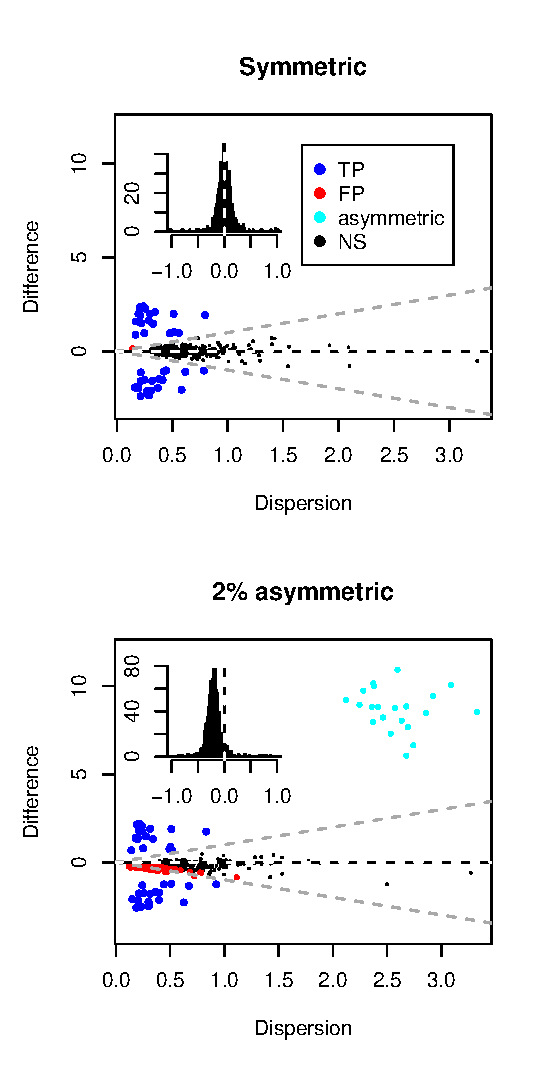
\includegraphics[scale=.65]{Fig_1-book.eps}
%
% If no graphics program available, insert a blank space i.e. use
%\picplace{5cm}{2cm} % Give the correct figure height and width in cm
%
\caption{Effect plots of simulated asymmetric data illustrates the problem.The effect plots show the difference between two conditions in simulated RNA-seq data with 1000 genes where 40 genes are modelled to have true difference between groups of an effect size of 1 or more. Each point is a feature (gene) and they are coloured in black if not different between groups. Red points indicate features that are false positive identifications, blue points indicate appropriate identification of the 40 true positive genes, and cyan indicates appropriate identification of the asymmetric features. The inset histograms show the distribution of the differences between groups as calculated by  \texttt{ALDEx2} , and the vertical line shows a difference of 0. These x-axis of each histogram is truncated to show only differences near the midpoint.}
\label{Fig:f1a}       % Give a unique label
\end{figure}



\subsection*{Four alternative methods}
\label{subsec:2.2}

In its initial implementation, \texttt{ALDEx2} computes the CLR, a per-sample geometric mean using all features as the baseline for feature comparisons. The `Symmetric dataset' panel in Figure \ref{Fig:f1a} is an `effect plot' \cite{gloor:effect} and we can see that that the 40 internal control features are found to be both statistically significant and to have an effect size greater than 1 between the two groups. The remainder of the features have very small difference and a very large dispersion, and correspondingly have an effect size much less than 1; that is, the results are as expected. 

% For figures use
%
\begin{figure}[b]
\sidecaption[t]
% Use the relevant command for your figure-insertion program
% to insert the figure file.
% For example, with the graphicx style use
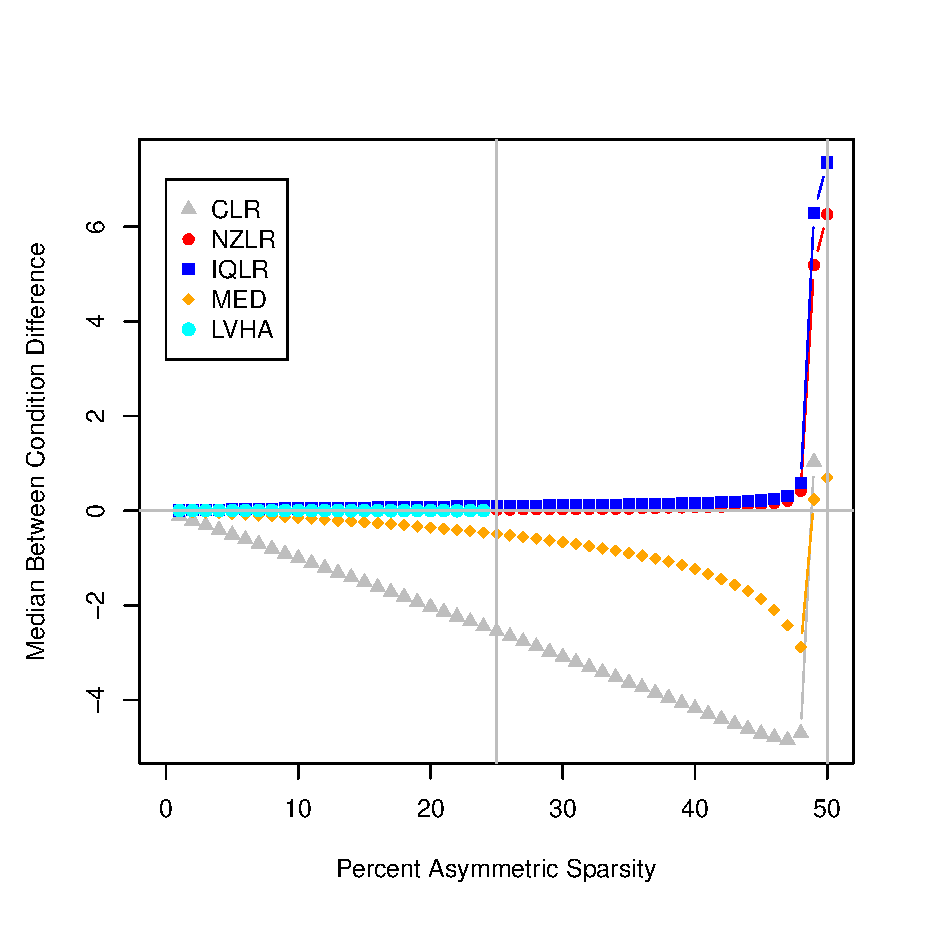
\includegraphics[scale=.45]{Fig_failure-book.eps}
%
% If no graphics program available, insert a blank space i.e. use
%\picplace{5cm}{2cm} % Give the correct figure height and width in cm
%
\caption{The behaviour of each transform for datasets with varying asymmetry. Each point represents the median between condition difference for a given transformation in a dataset with a specified sparsity. Points closer to the location y=0 are favourable and indicate proper centring of the dataset. Abbreviations for each method for determining the denominator are the same as in the text.}
\label{Fig:f2a}       % Give a unique label
\end{figure}



The inset histogram shows that the distribution of difference values between groups A and B is symmetric and has a location of 0. However, the introduction of small amounts of asymmetry strongly affect the results. The asymmetric 2\% dataset is the base dataset modified by choosing 20 randomly  features from Group A and setting their value to 0. It is apparent from the bottom  panel of Figure \ref{Fig:f1a} that even this low level of simulated asymmetry breaks the assumption that most features are invariant, and the location of  modal no-difference between groups is no longer at the origin.  This small amount of asymmetry  shifts the geometric mean of the data such that the two groups are calculated using systematically different denominators, causing bias. It is unlikely that the problem will be as easy to diagnose in real data as in simulated data. 

The major determinant of the centre of a sample when using the CLR is the denominator used to compute the CLR, thus, one obvious approach to address the problem is to compute the geometric mean of a subset of features that are more representative of the central tendency of those features in the dataset that are relatively invariant, and to use this geometric mean as the denominator. We  examined four different approaches to identifying the features to include in the denominator, and tested them with different proportions of modelled sparse asymmetry.

The transformation in Equation \ref{eq:iqlr} is termed the IQLR transformation, and relies on finding those features with `typical' variance in the dataset. The assumption being made here is that features with typical variance are those that do not differ between groups, but whose variance arises through stochastic processes in either sampling, sequencing or processing. The results of this method are shown in Figure \ref{Fig:f2a}, and we see that the IQLR transformation restores the centre of the dataset to the origin even when over 40\% of the modelled features are asymmetric.

The second approach uses as the denominator the set of non-zero features in each group calculated as in equation \ref{eq:nzlr}.  Thus, in this case the geometric mean of group A and group B are based on different, but potentially overlapping, sets of features, this approach is called the non-zero log ratio (NZLR), and is similar in concept to another recent approach \cite{Martino:2019aa}. As shown in Figure \ref{Fig:f2a} the NZLR method also restores the centre of the data to the origin with similar efficiency in our test dataset as does the IQLR method. Note that if the asymmetry is not driven by sparsity, the NZLR method method will obviously fail. This method is not recommended unless the investigator knows from prior inspection  that asymmetric sparsity occurs.   The \texttt{zCompositions R} package contains convenient functions to explore sparsity in compositional data \cite{PalareaAlbaladejo201585}.

The third approach was to identify the intersect between groups of those features that have variance which is in the bottom quartile  and a relative abundance in the top quartile in each group. This is referred to as the low variance high abundance log ratio  \textit{LVHA} method and is calculated as in equation \ref{eq:lvha}. In essence, the LVHA approach is an attempt to identify those features that would be similar to those chosen by an experimentalist using qPCR; being relatively abundant with low variance in all groups in the dataset.  The results of this method are shown in Figure \ref{Fig:f2a}. We can see that the LVHA approach perfectly centres the data up to 25\% asymmetry in our test dataset.  

The fourth approach replaces the geometric mean in Equation \ref{eq:CLR} with the  median of the vector as in equation \ref{eq:med} since this should be a robust estimate of the midpoint of the data. We can see in Figure \ref{Fig:f2a} that the median is better than the geometric mean at low proportions of asymmetry, but performs worse than the previous approaches in almost every case.

\subsection*{Example of a meta-RNA-seq dataset}
\label{subsec:2.3}


 We finally introduce the example of a real meta-transcriptome dataset collected to determine the differences in gene expression of the vaginal microbial community in the healthy (H) and bacterial vaginosis (BV) states \cite{macklaim:2013,Denge00262-18}. The vaginal community can be dominated either by a few members of the \textit{Lactobacillus} genus in the H state, or by a mixed group of anaerobic bacterial genera in the BV state \cite{Ravel:2010}. In either state the members of the bacterial consortium from the other state are either very rare or absent. The data presented in Figure \ref{Fig:f3a} show effect size plots for the CLR and three different demonimators for a count table  derived from data deposited at the European Nucleotide Archive metagenomics site under the accession number PRJEB31833 using  the  methods in \cite{Macklaim:2018aa} and annotated using the SEED subsystems \cite{Overbeek:2014aa}. Compatible count tables for other metatranscriptomic or metagenomic datasets may be downloaded from the EBI metagenomics web site \cite{Mitchell:2018aa}.

% For figures use
%
\begin{figure}[!b]
\sidecaption[t]
% Use the relevant command for your figure-insertion program
% to insert the figure file.
% For example, with the graphicx style use
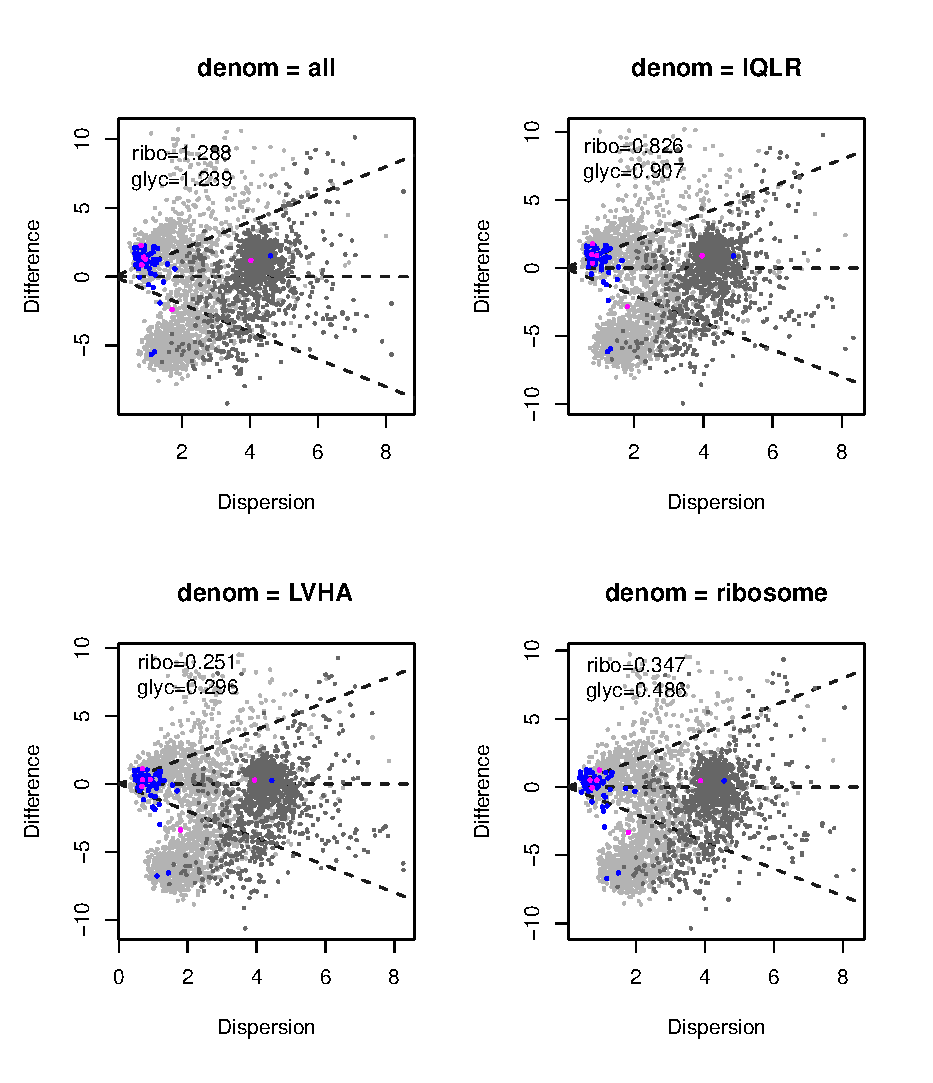
\includegraphics[width=10cm]{MAx4-book.eps}
%
% If no graphics program available, insert a blank space i.e. use
%\picplace{5cm}{2cm} % Give the correct figure height and width in cm
%
\caption{Sparsity and asymmetry in a meta-transcriptome dataset of vaginal samples.  The panel show effect plots with log base 2 scaling of the data using the log-ratio values. Each point is a SEED-level 4 functional annotation category derived from the raw reads as in \cite{Macklaim:2018aa} and they are coloured in light grey if no sample contains a 0 value (non-sparse), dark grey if at least one sample contains a 0 count, blue if annotated as a protein translation function or magenta if annotated as a glycolytic function. The median displacement of the functional subsets from 0 is given in the top left of the plot.  The user-defined denominator was composed of functions annotated as ribosomal small or large subunit functions.  }
\label{Fig:f3a}       % Give a unique label
\end{figure}

  
The values in Figure \ref{Fig:f3a}:denom=all were computed using the CLR. We can see that there is a large asymmetry in distribution, the most striking of which are the functions in BV located below the midline on the y-axis. This asymmetry is driven by the greater complexity of the BV microbial community, and the generally larger and more complex genomes in the set of bacteria found in BV \cite{macklaim:2013}. The asymmetry is composed of both presence-absence (sparsity) and large differences between groups. This can be seen with the sparsity overlay color, where functions that contain one or more zeros are coloured in a dark grey. 

Note that there appears to be two clusters of functions that are just above the y-axis midline. The ones at location [x=4, y=2] are composed of sparse functions expressed at low levels in BV but that are absent or very rare in H.  We also see a second group composed of functions found in common between the the H and BV group that is  expressed at very high relative levels, centred around location [x=1, y=1.5] on the  plot. These are generally housekeeping functions that are central and required by all living organisms, and we can see that the two sets of housekeeping functions that are  highlighted cluster here: translational protein functions in blue (rib), and glycolysis (glycolic, core sugar metabolism) related functions in magenta. Many of the functions in these groups are often used as internal standards for comparison by qPCR as it is assumed that their expression is invariant \cite{Scott:2010}, and we are attempting to minimize the displacement of these functions from a difference location of 0 . The median offset of the two sets of housekeeping functions  on the y-axis is given, and we can see that they are both observed to be substantially above the expected location of 0 when the CLR alone is used to determine differential relative abundance.   

The other three panels in Figure \ref{Fig:f3a} shows the result of applying  three adjustment approaches to the asymmetric meta-RNA-sea dataset. The LVHA, IQLR and user-defined-adjustment (ribosome) methods all centred the data  better than did the CLR. In the case of the user-defined functions we used the set of translational protein functions in blue as the denominator in the denom=ribosomal panel. We can see that the bulk of the expected invariant groups are closer to the y-axis midline with two adjustments, and the offset of the translational and glycolytic functions is reduced substantially when compared to the CLR result. The LVHA adjustment brings the housekeeping functions very close to the centre of the dataset.  Centring on the geometric mean of the low variance but high (relative) abundance functions provides a substantial improvement over all other methods in this dataset.

\section*{Discussion}

Biological data derived from high-throughput sequencing is rarely ideal and exhibits many pathologies. It is currently difficult to examine complex communities using RNA-seq because of a mismatch between the assumptions of the tools and the characteristics of the data. In particular, such data can be derived from asymmetric environments, where sets of genes, operational taxonomic units, or organisms can be present or abundant in one condition and absent or rare in another. Asymmetries also often exist in metagenomic, and in vitro selection (SELEX) datasets, and the approaches described here help to recenter the data  \cite{Almeida:2019aa,McMurrough:2018aa,Wolfs:2016aa}.  Alternatively, an asymmetry in the data can arise because of a systematic failure in experimental design, for example, through improper blocking or the presence of outlier samples. In any of these instances the presence of an asymmetry may not be obvious. 

In a biological context it is entirely reasonable that asymmetry could occur because counts  rather than simple sparsity. For example, the default gene expression condition for many genes is low-level expression, and the inclusion of a transcriptional activator could increase expression of many genes from very low expression to very high expression. In the context of 16S rRNA gene sequencing study, it is possible for samples to be dominated by one very abundant organism but to contain many other taxa at low abundance. Thus, we would have a count asymmetry that is not necessarily based on sparsity, and for this reason we do not recommend the NZLR approach unless the others fail. Furthermore, sparsity is strongly affected by read depth, the same samples derived from a sequencing dataset from an Illumina NextSeq run delivering a total count of 400M reads will be substantially less sparse than those derived from an Illumina MiSeq run delivering a total count of 25M reads, however any underlying asymmetry will be preserved.

We demonstrated that even a small number of asymmetric features can change the location of the dataset, leading to both false positive and false negative differences being identified. When the asymmetry is moderate, the IQLR correction is most appropriate. This correction makes the assumption that those features with variance between the first and third quartile of variance are a suitable proxy for the expected `typical' variance of the data. This approach can tolerate up to at least 40\% asymmetry in the data when the geometric mean of these features are used as the denominator for a log-ratio normalization. Both the NZLR and the IQLR break down when the asymmetry exceeds about 45\%, and this breakdown becomes severe above 48\% asymmetry. This reason for this is unknown. However, we recommend that the IQLR be used as the default when performing differential relative abundance analysis, since this normalization makes no strong assumption about the data and appears to never perform worse than the CLR normalization until failure of the approach occurs. In this case \texttt{ALDEx2} will report an error.

% For figures use
%
\begin{figure}[b]
\sidecaption[t]
% Use the relevant command for your figure-insertion program
% to insert the figure file.
% For example, with the graphicx style use
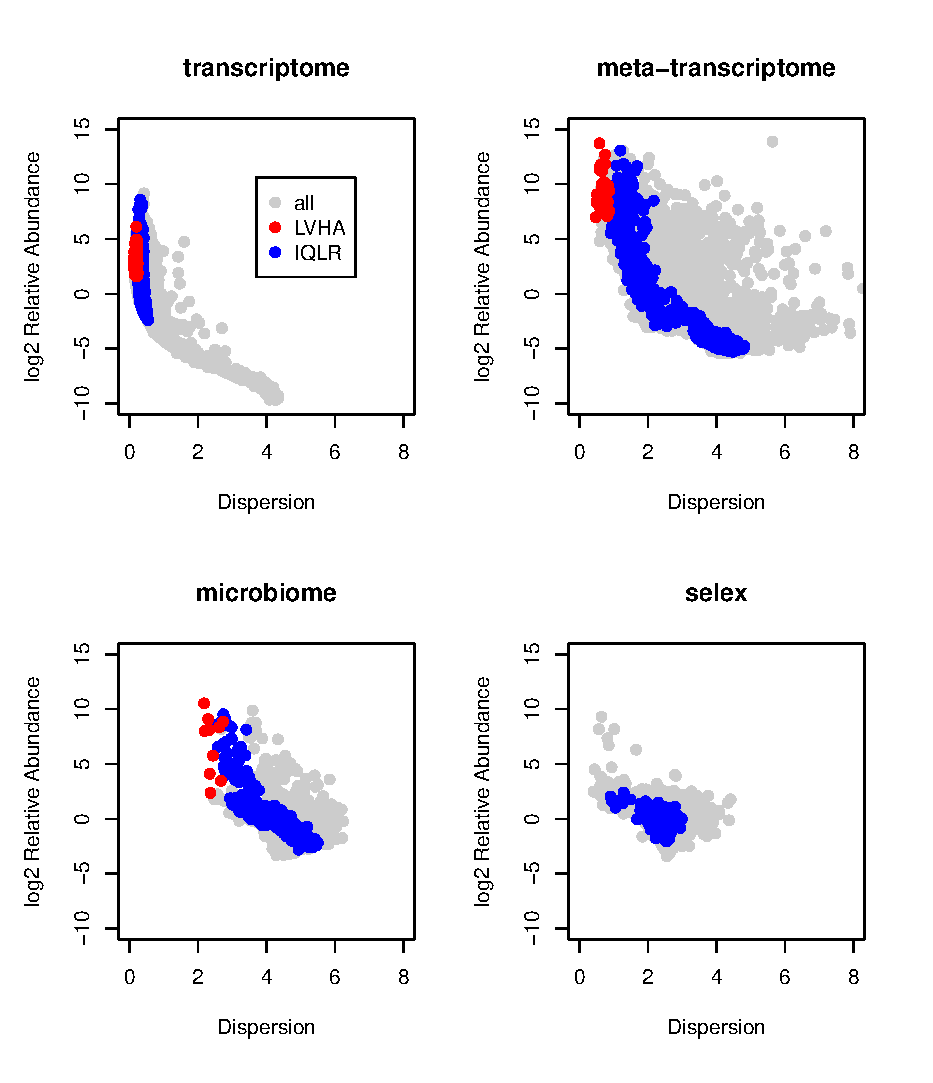
\includegraphics[scale=.45]{Disp-v-Abund.eps}
%
% If no graphics program available, insert a blank space i.e. use
%\picplace{5cm}{2cm} % Give the correct figure height and width in cm
%
\caption{Variance and abundance relationships for four different types of data. The x-axis plots data from the \texttt{rab.all} column and the y-axis plots the \texttt{diff.win} column  output by \texttt{aldex.clr}. The denominators used by the CLR, IQLR and LVHA methods are outlined as given in the legend.  The transcriptome dataset is an ideal RNA-seq dataset that shows a very strong relationship between these two measures. The relationship between these measures is not as strong in the meta-transcriptome dataset but some relationship is easily discernible. The microbiome and selex datasets have a very poor variance-abundance relationship. }
\label{Fig:varabund}       % Give a unique label
\end{figure}

More extreme asymmetry, as found in the vaginal transcriptome dataset, forces the investigator to make strong assumptions about the underlying data and use the LVHA correction, or to explicitly choose a set of housekeeping genes. The assumptions made here are thus similar to the assumptions made when performing qPCR: that there are one or more invariant features in the data, and that these will typically be relatively abundant house-keeping functions. We found that these features could usually be identified as having low variance but high relative abundance and can be used as exemplars of `invariant' features. 

When choosing between methods it can be instructive to examine the variance-abundance relationship of the data. Figure \ref{Fig:varabund} shows these relationships for four different types of datasets, and we can see that the relationship is very different for each type of data. When the variance-abundance relationship is very tight (even if non-linear), the LVHA method is generally preferred as in the transcriptome \cite{Gierlinski:2015aa} and meta-transcriptome datasets. Here, it is relatively simple to make a case for the biological meaning of the LVHA method, as it is identifying 'cellular housekeeping' features that are assumed to be relatively invariant \cite{Scott:2010}. When conducting qPCR, these (or a subset) are the set of features that the experimentalist chooses as a reference. However, when analyzing a microbiome \cite{bian:2017}, or in-vitro selection experiment (selex) \cite{mcmurrough:2014}, we can see that the variance-abundance relationship is very poorly defined. In these experimental design, it is difficult to argue that any set of features should have both high abundance and low variance, and indeed we observe that the number of features in the LVHA denominator is low or absent. In contrast, we observe that the IQLR approach is more general in nature and features fulfilling the requirements of equation \ref{eq:iqlr} are more easily met. Thus, in general the IQLR approach is preferred unless the experimentalist has strong information about the underlying nature of the dataset. 

 
\section*{Conclusions}
We tested  different methods to  centre the data, and found that the IQLR and LVHA-specified centring approaches were the most general purpose and thus recommended for use. All are implemented in the \texttt{ALDEx2} R package \cite{fernandes:2014} and can be used in conjunction with the \texttt{propr} R package for compositional association \cite{Quinn:2017}.   In any case, it must be remembered that the results of any analysis must be interpreted as \textit{abundance relative to the chosen invariant part of the dataset}, and not as changes in absolute abundance.

\section*{Abbreviations}

\noindent ALR: additive log-ratio transformation

\noindent BA plot: Bland-Altman plot

\noindent BV: bacterial vaginosis state

\noindent CLR: centred log-ratio transformation

\noindent H: healthy (non-BV) state

\noindent HTS: high throughput sequencing

\noindent IQLR: the inter-quartile log-ratio method

\noindent LVHA: the low variance, high abundance method

\noindent M: million

\noindent NZLR: the non-zero log ratio method

\noindent OTU: operational taxonomic unit

\noindent qPCR: quantitative PCR

\section*{Declarations} 

\section*{Availability and requirements}

The methods are included in the \texttt{ALDEx2} R package available at Bioconductor (https://www.bioconductor.org/packages/release/bioc/html/ALDEx2.html). 

\subsection*{Ethics approval and consent to participate}
Not applicable

\subsection*{Consent for publication}
Not applicable

\subsection*{Availability of data and material}
All data used in this publication are publicly available. The raw data for the yeast genome was drawn from the reference \textit{Saccharomyces cerevisiae} genome at: https://www.ncbi.nlm.nih.gov/genome/?term=txid4932. were generated from the data  The raw data for Figure 3 was obtained from European Nucleotide Archive metagenomics site under the accession number PRJEB31833 using  the  methods in \cite{Macklaim:2018aa}. Additional data for the tables of counts in Figure 4 were from the following: \cite{mcmurrough:2014,Gierlinski:2015aa,bian:2017}. All R scripts for figure generation and analysis are located on a public GitHub repository at: https://github.com/ggloor/working-papers/Festschrift.

\subsection*{Competing interests}
The authors declare that they have no competing interests.
  
\subsection*{Funding}
This work was supported by a grant from the Natural Sciences and Engineering Research Council of Canada grant RGPIN-2015-03878 to GBG

\section*{Author's contributions}
 Designed the experiments GBG, JMM, JRW, BLG. Developed and applied corrections BLG, JRW, GBG, JMM. Wrote the manuscript, GBG. All authors have read and approved the manuscript.

\section{Competing interests}

None of the authors declare competing interests.

\subsection*{Acknowledgements}
GBG first met Dr. Palwlowsky-Glahn in 2014 where she was an instructor and organizer of the CoDa summer school. At that time our group was struggling with interpreting meta-transcriptomic datasets, and found that compositional approaches were promising. GBG thanks Vera for her everlasting patience in answering any and all questions, and for making the entry into the world of CoDa a fruitful and rewarding experience.

\bibliographystyle{spmpsci} % Style BST file (bmc-mathphys, vancouver, spbasic).
%\bibliography{bibdesk_refs.bib}
\bibliography{Gloor-F.bbl}
%\input{references}
\end{document}
